\begin{figure}[htbp]
    \centering
    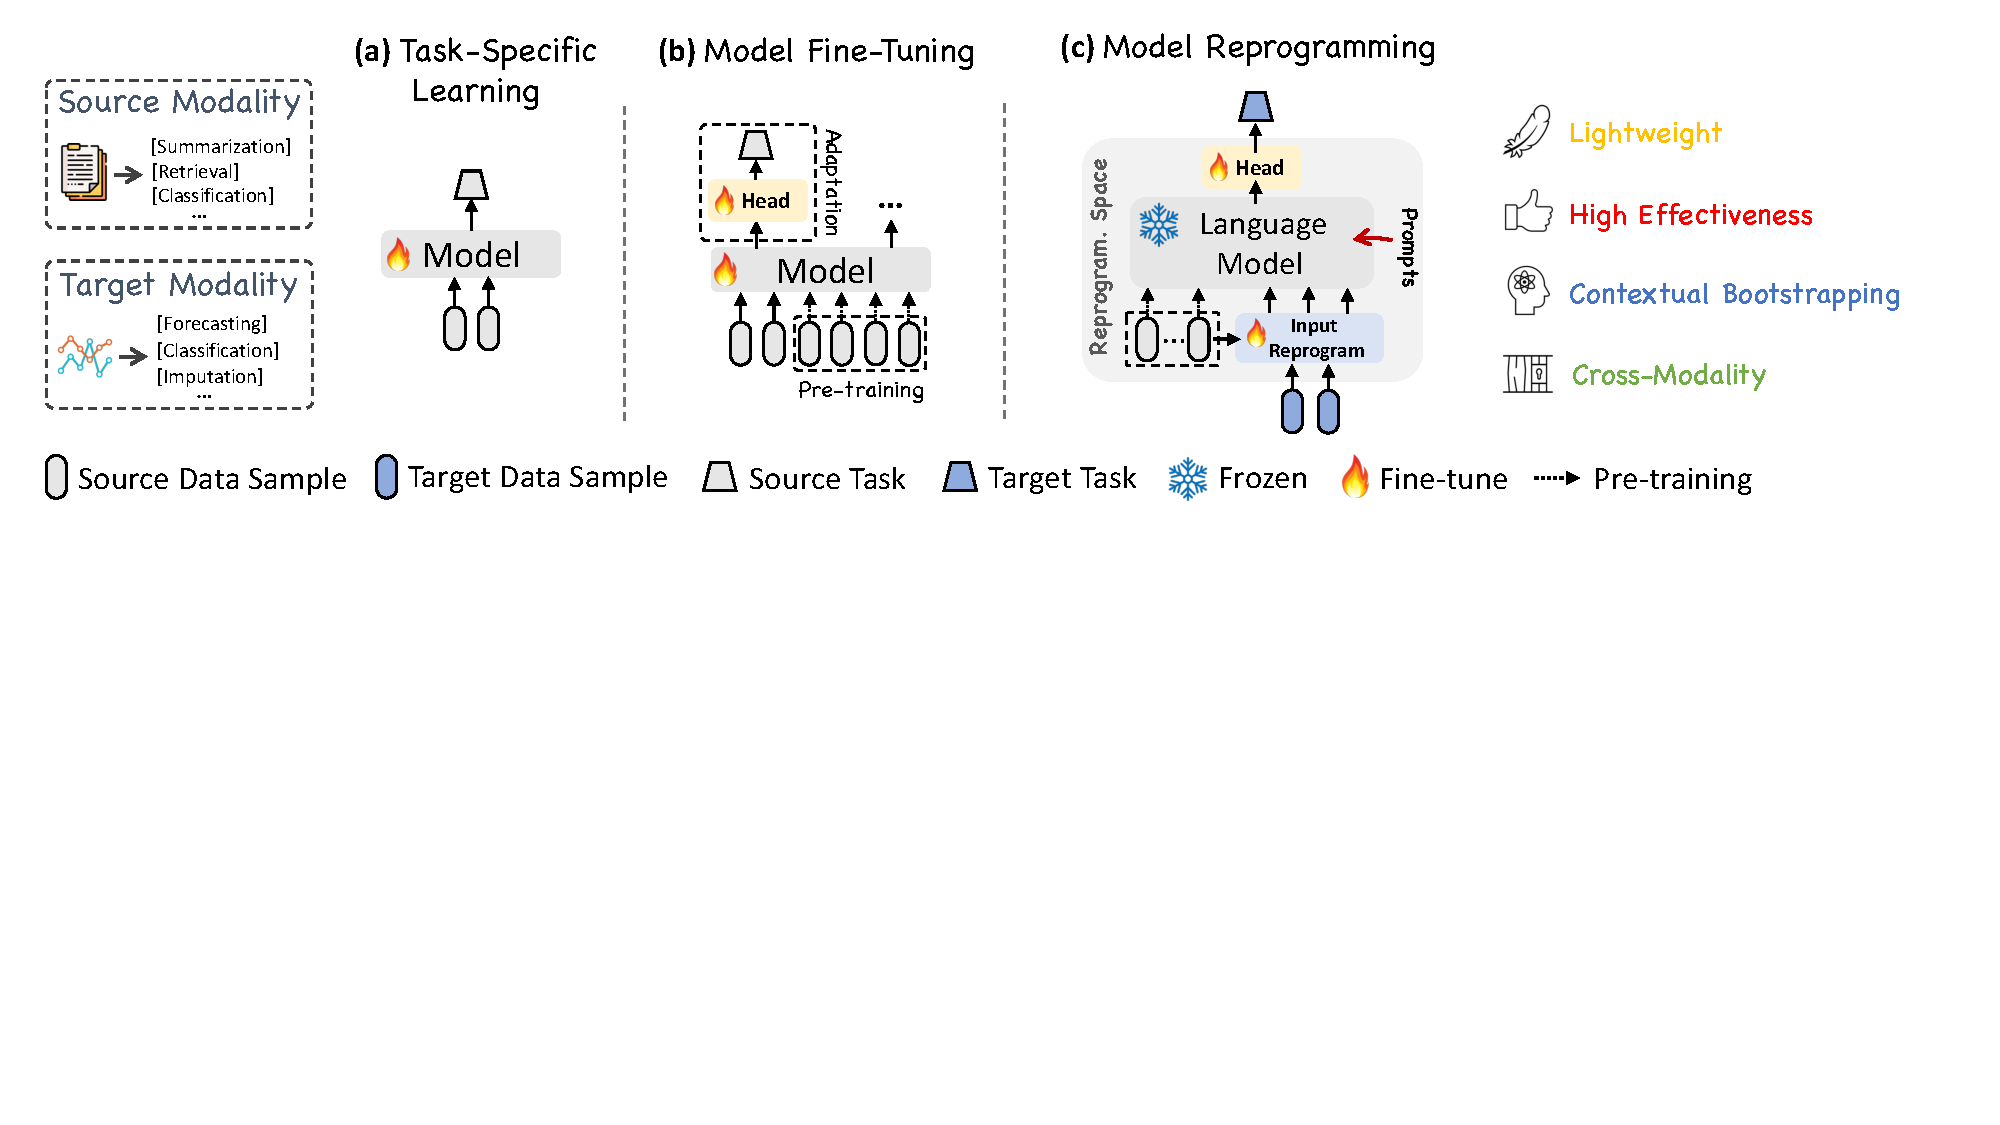
\includegraphics[width=0.99\textwidth]{figures/schematic_illustration_v5.pdf}\vspace{-2mm}
    \caption{Schematic illustration of reprogramming large language models (LLMs) in comparison of \textbf{(a)} task-specific learning and \textbf{(b)} model fine-tuning. Our proposal investigates and demonstrates \textbf{(c)} how to effectively reprogram open-sourced LLMs as powerful time series learners where well-developed time series pre-trained models are not readily available.
    }
    \vspace{-5mm}
    \label{fig:schematic}
\end{figure}

\noindent\textbf{Task-specific Learning.} Most time series forecasting models are crafted for specific tasks and domains (e.g., traffic prediction), and trained end-to-end on small-scale data. An illustration is in \shortautoref{fig:schematic}(a). For example, ARIMA models are designed for univariate time series forecasting~\citep{box2015time}, LSTM networks are tailored for sequence modeling~\citep{hochreiter1997long}, and temporal convolutional networks~\citep{bai2018empirical} and transformers~\citep{wen2023transformers} are developed for handling longer temporal dependencies. While achieving good performance on narrow tasks, these models lack versatility and generalizability to diverse time series data.

\noindent\textbf{In-modality Adaptation.} 
Relevant research in CV and NLP has demonstrated the effectiveness of pre-trained models that can be fine-tuned for various downstream tasks without the need for costly training from scratch \citep{devlin2018bert,brown2020language,touvron2023llama}. Inspired by these successes, recent studies have focused on the development of time series pre-trained models (TSPTMs). The first step among them involves time series pre-training using different strategies like supervised~\citep{fawaz2018transfer} or self-supervised learning~\citep{zhang2022self,deldari2022beyond,zhang2023self}. This allows the model to learn representing various input time series. Once pre-trained, it can be fine-tuned on similar domains to learn how to perform specific tasks~\citep{tang2022domain}. An example is in \shortautoref{fig:schematic}(b). The development of TSPTMs leverages the success of pre-training and fine-tuning in NLP and CV but remains limited on smaller scales due to data sparsity.

\noindent\textbf{Cross-modality Adaptation.} Building on in-modality adaptation, recent work has further explored transferring knowledge from powerful pre-trained foundations models in NLP and CV to time series modeling, through techniques such as multimodal fine-tuning~\citep{yin2023survey} and model reprogramming~\citep{chen2022model}. Our approach aligns with this category; however, there is limited pertinent research available on time series. An example is Voice2Series~\citep{yang2021voice2series}, which adapts an acoustic model (AM) from speech recognition to time series classification by editing a time series into a format suitable for the AM. Recently, \cite{chang2023llm4ts} proposes LLM4TS for time series forecasting using LLMs. It designs a two-stage fine-tuning process on the LLM - first supervised pre-training on time series, then task-specific fine-tuning. \cite{zhou2023one} leverages pre-trained language models without altering their self-attention and feedforward layers. This model is fine-tuned and evaluated on various time series analysis tasks and demonstrates comparable or state-of-the-art performance by transferring knowledge from natural language pre-training. Distinct from these approach, we neither edit the input time series directly nor fine-tune the backbone LLM. Instead, as illustrated in \shortautoref{fig:schematic}(c), we propose reprogramming time series with the source data modality along with prompting to unleash the potential of LLMs as effective time series machines.